\section{NN and Bayesian NN}\label{sec:bnn}
\subsubsection{Neural Networks}
\textit{Neural Networks} are deep, supervised, discriminative models, which consist of at least two connected layers of nodes—input and output, and usually with one or more hidden layers in between (see \autoref{fig:bnn-dnn-point-estimate}). In \autoref{fig:bnn-dnn-neuron} a visualization of a neuron is presented. Each neuron has weights $w$ incoming from inputs $x$ of the previous layer (with an addition of a bias term $b$), and an activation function $f$, which yields an output $z$.

\begin{figure}[h]
     \centering
     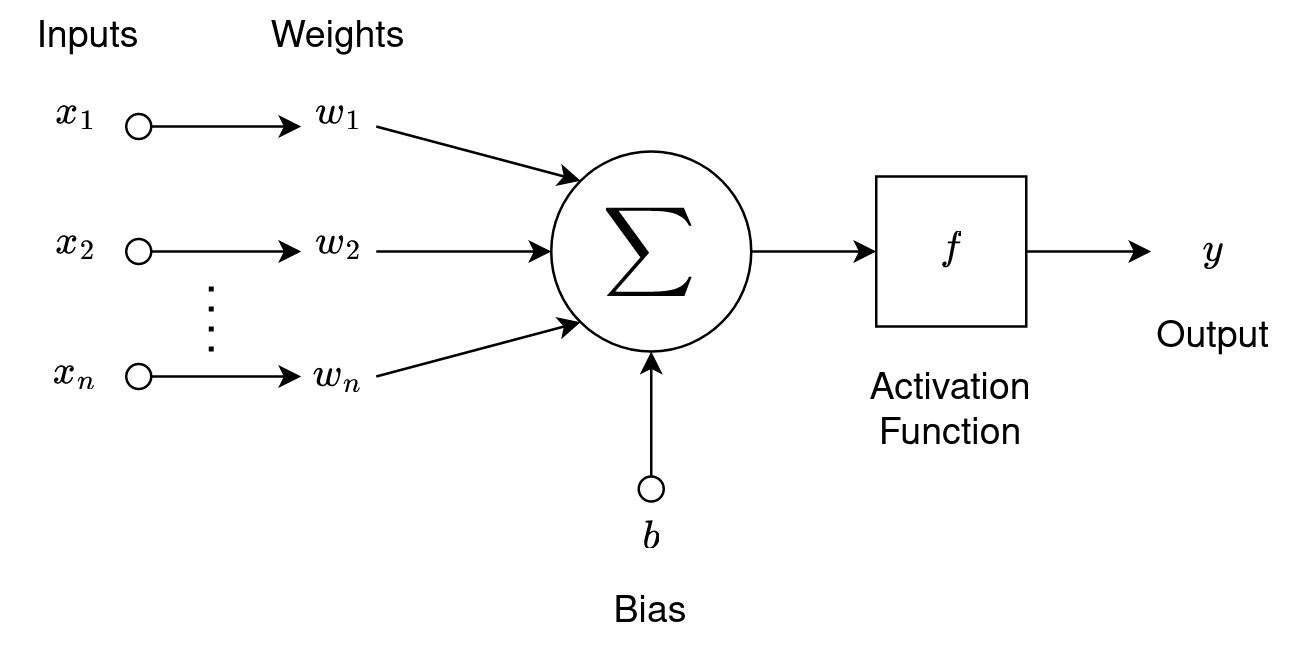
\includegraphics[width=0.9\textwidth]{methods/img/DNN_neuron.drawio.png}
     \caption[A DNN neuron]{A visualization of a Deep Neural Network's neuron.}
    \label{fig:bnn-dnn-neuron}
\end{figure}

\noindent This way, weights of the current node are a linear transformation of the previous one. It can be denoted as follows:
\begin{equation}
    z^{(i+1)} = W^{(i+1)}x^{(i)} + b^{(i+1)}
\end{equation}

\noindent In the deterministic setting, weights directly correspond to trainable parameters. They are optimized with a backpropagation algorithm that uses gradient descent to optimize the cost function or the error of the model. This results in point estimates of the weights, which is visualized in \autoref{fig:bnn-dnn-point-estimate}.

\begin{figure}[h]
     \centering
     \begin{subfigure}[b]{0.45\textwidth}
         \centering
         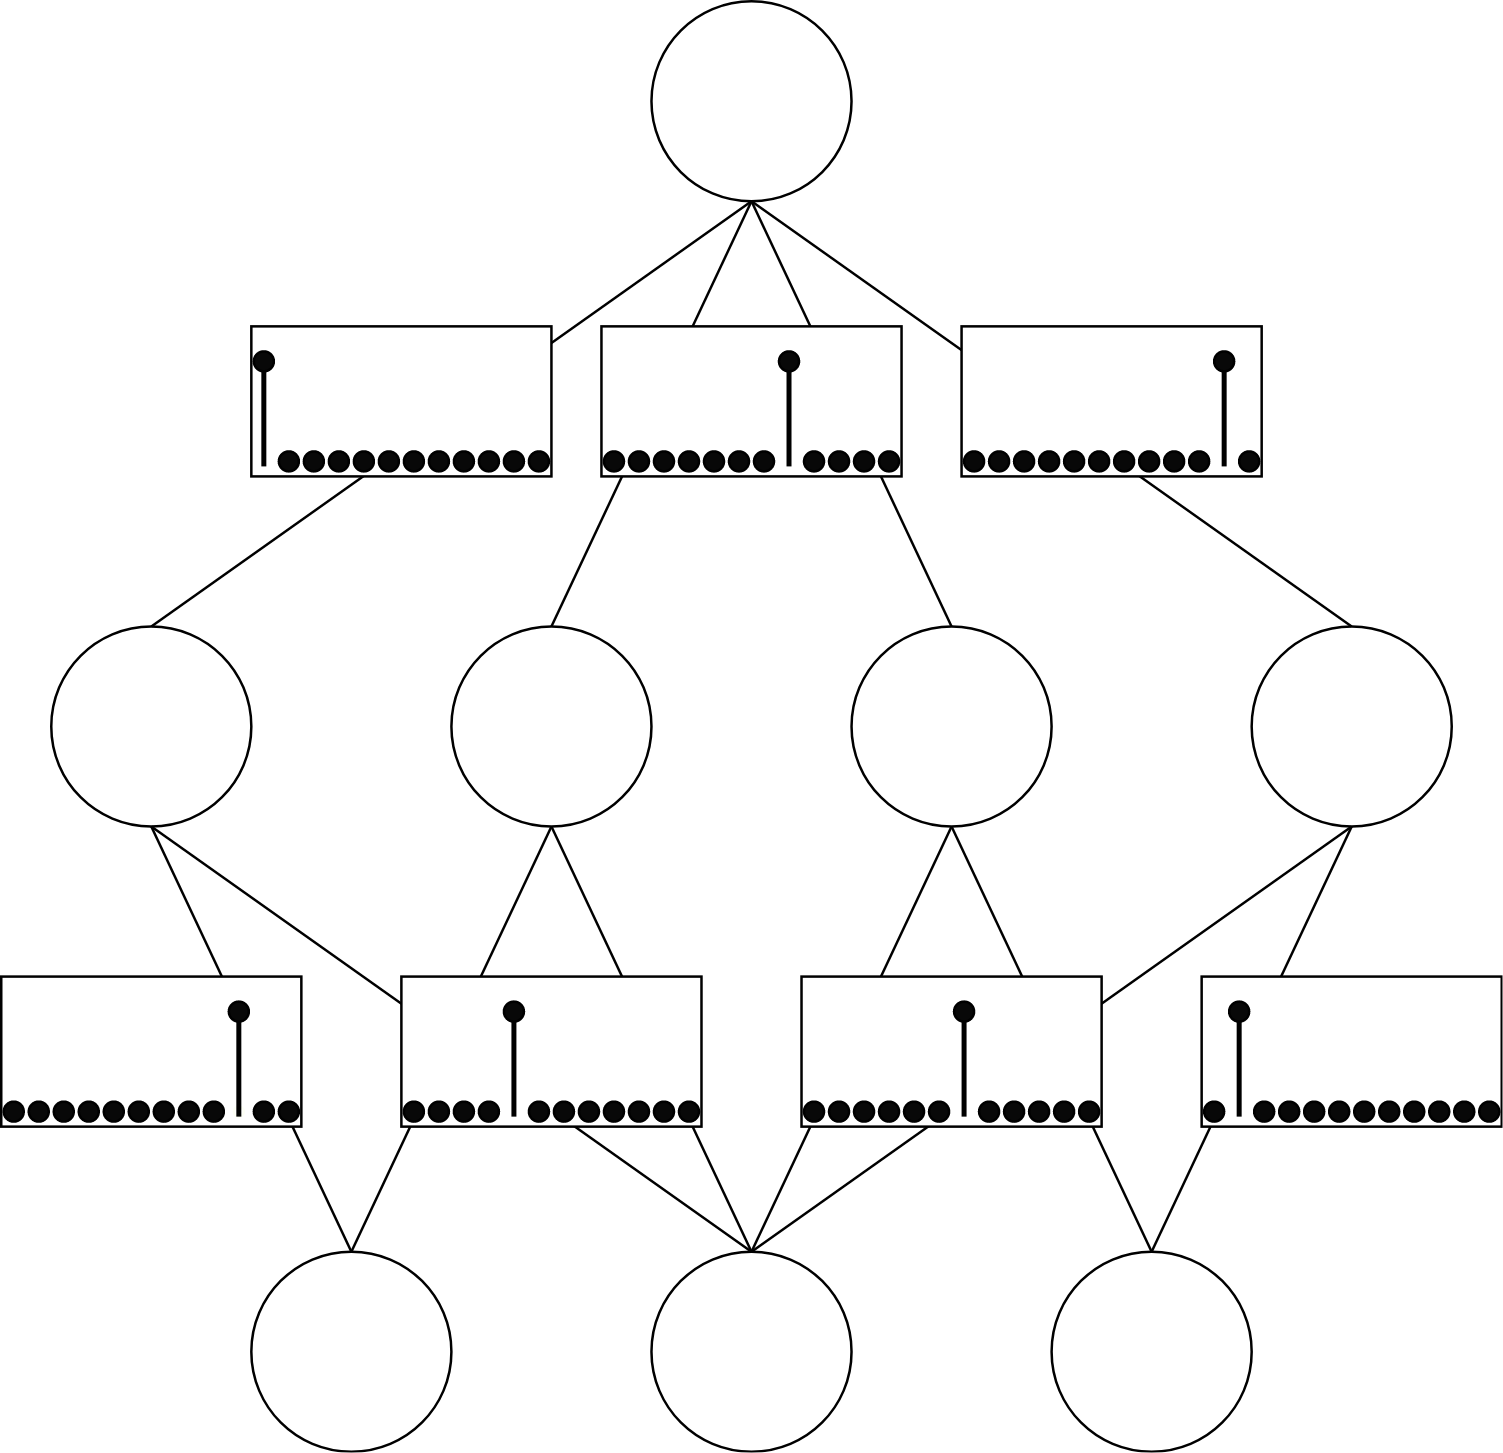
\includegraphics[width=\textwidth]{methods/img/DNN.drawio.png}
         \caption{DNN with point estimates} \label{fig:bnn-dnn-point-estimate}
     \end{subfigure} 
     \hfill
     \begin{subfigure}[b]{0.45\textwidth}
          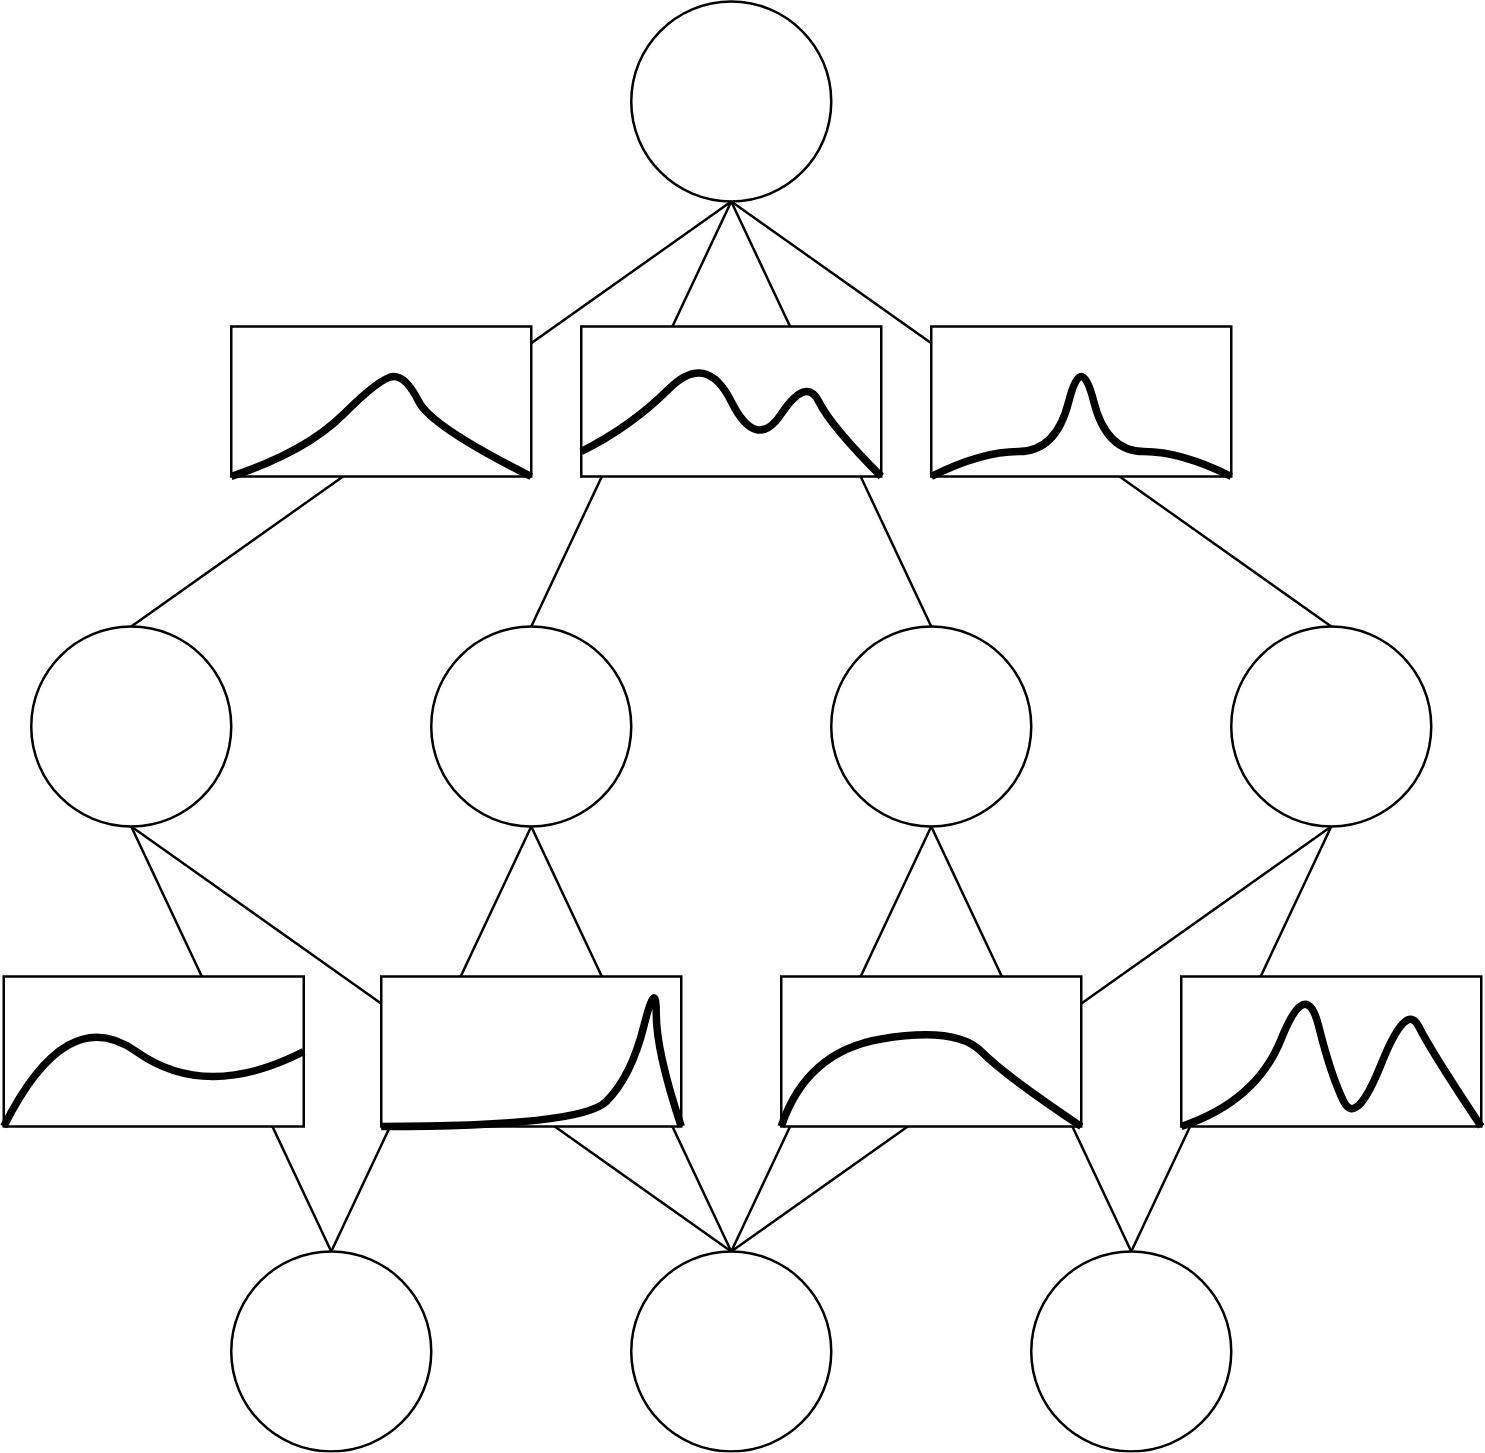
\includegraphics[width=\textwidth]{methods/img/BNN.drawio.png}
         \caption{BNN with distributions over weights} \label{fig:bnn-distribution-estimate}
     \end{subfigure} 
     \caption[Comparison of DNN and BNN approaches]{A comparison of Deep Neural Network point-estimate (a) and Bayesian Neural Network (b) distributions-over-weights approaches.}
    \label{fig:bnn-dnn-approaches}
\end{figure}


\vspace{\baselineskip}
Conventional neural networks, do come with certain disadvantages. They tend to be miscalibrated, and thus overconfident in their predictions \cite{Guo2017}. \say{A neural network can represent many models consistent with our observations. By selecting only one, in a classical procedure, we lose uncertainty when the models disagree for a test point} \cite{Wilson2020}.


\subsubsection{Bayesian Neural Networks}
\textit{Bayesian Neural Networks} (BNN) is a family of methods that extend conventional neural networks with Bayesian inference of posterior distributions on parts of their architecture, most often either weights (see \autoref{fig:bnn-distribution-estimate}) or activation functions. They are sometimes described as neural networks with stochastic elements trained in a Bayesian framework \cite{MacKay1992}. Introducing the Bayesian factor results in certain advantages with the conventional approach.

\vspace{\baselineskip}
The most important is a realistic expression of uncertainty and calibration. Gathering the uncertainty helps to reduce the network's variance over the prediction of a specific data point. It provides an edge of being able to assess the model quality not only in terms of how many times it was wrong, but also by how much. Additionally, because of the Bayesian setting, it is possible to encode a priori knowledge about the network parameters. In certain situations, it results in less complex learning of more accurate models.

\vspace{\baselineskip}
Considering how convoluted the concepts of neural networks and Bayesian approaches are, it is surprisingly how simple it is to combine both of them. There is a wide range of possible approaches to designing a functioning model. Because of the multiplicity of possibilities, the following paragraphs will focus only on the approach adopted in this work.

\paragraph{Bayes by Backprop}\label{paragraph:bayes-by-backrop}
\textit{Bayes by Backprop} (BBB) \cite{Blundell2015} is a method from the variational inference family that is adapted for neural networks. In its essence, it is supposed to replace conventional backpropagation (thus its name) with learning the parameters of an approximate posterior by unbiased Monte Carlo estimates of the gradients.

\vspace{\baselineskip}
In this setting, a stochastic neural network can be seen as an ensemble model, in which each network can be drawn from a common and learned probability distribution by sampling the weights. The exact Bayesian inference on the weights of a neural network is intractable (due to a large space of parameters). Because of that, the goal is to find parameters $\theta$ that minimize the Kullback-Leibler divergence between the variational distribution $q(w \mid \theta)$ and the posterior $P(w \mid D)$:

\begin{equation}\label{eq:bnn-kl-divergence-transformation}
\begin{split}
    \theta_{opt} &= \text{arg min}_\theta\; D_{KL}\left[q(w \mid \theta) \parallel P(w \mid D) \right] \\
    &= \text{arg min}_\theta \int q(w \mid \theta) \log\frac{q(w \mid \theta)}{P(w)\:P(D \mid w)}\, dw\\
    &= \text{arg min}_\theta\; D_{KL}\left[q(w \mid \theta) \parallel P(w) \right] - {\mathbb{E}}_{q(w \mid \theta)}\left[log\:P(D \mid w)\right],
\end{split}
\end{equation}

\noindent where $w$ are the weights. In order to obtain the unbiased estimates of the gradients, a Monte Carlo simulation can be performed. Then, the optimal weights are as follows:

\begin{equation}\label{eq:bayes-by-backprop-loss}
     \theta_{opt} = \text{arg min}_\theta \frac{1}{N} \sum^{n}_{i=1}log\:q(\mathbf{w}^{(i)} \mid \theta) - log\:P(\mathbf{w}^{(i)}) - log\:P(D \mid \mathbf{w}^{(i)}),
\end{equation}

\noindent where $\mathbf{w}^{(i)}$ denotes the $i$-th Monte Carlo sample drawn from the variational posterior $q(\mathbf{w}^{(i)} \mid \theta)$, and $N$ is the number of Monte Carlo estimations. Note that the last term - $log\:P(D \mid \mathbf{w}^{(i)})$ is a likelihood function of the conventional neural network.

\paragraph{Reparameterization trick}
As a consequence of the sampling procedure being indifferentiable, the parameter optimization process requires reparameterization \cite{Kingma2015}. To obtain the weight $w$, if assuming a Gaussian, every learnable parameter will be defined by the parameters of this distribution — mean $\mu$ and variance $\sigma^2$, then:
\begin{equation}
    \theta = \mu + \sigma + \epsilon,
\end{equation}

\noindent where $\epsilon$ is noise and $\epsilon \sim \mathcal{N}(0, 1)$. It is also the only intractable element. Because, however, only $\mu$ and $\sigma$ are important, it can be skipped. In such manner, gradients can be induced:
\begin{align}
    \Delta_\mu &= \frac{\partial f}{\partial \theta} + \frac{\partial f}{\partial \mu} \\
    \Delta_\sigma &= \frac{\partial f}{\partial \theta} \frac{\epsilon}{\sigma} + \frac{\partial f}{\partial \sigma}.
\end{align}

\noindent Parameters are updated the following way:
\begin{align}
    \mu^{(t+1)} &= \mu^{t} - \alpha \Delta_\mu \\
    \sigma^{(t+1)} &= \sigma^t - \alpha \Delta_\sigma
\end{align}

\subsubsection{Representations}
Because neither DNN nor BNN defines representation explicitly, it might not seem obvious how to obtain it. This is, in fact, reasonably simple — the outputs of each layer of the network are a separate representation, and it is enough to extract it from there. While designing a network with representation learning in mind, it is important to consider the right architecture (for instance, dimensionality of the desired layer).


%  implementation - \cite{Esposito2020}